\documentclass[a4paper,11pt]{book}

\usepackage[T1]{fontenc}
\usepackage[utf8]{inputenc}
\usepackage{ragged2e}
%\usepackage{mathtools}makeglossaries %.tex
\usepackage{graphicx}
\usepackage[margin=1in]{geometry}
\usepackage[spanish, es-tabla, es-noquoting]{babel}
\usepackage[hidelinks]{hyperref}
\usepackage{fancyhdr}
\usepackage{incgraph,tikz}
%\usepackage{caption}
\usepackage{subcaption}
\usepackage{amsfonts}
%\usepackage{babel}
\usepackage{color}
\usepackage{listings}
\usepackage{float}
\usepackage{tikz}
\usepackage{adjustbox}
\usepackage[numbers,square]{natbib}
\usepackage{xcolor}
\usepackage{titlepic}
\usepackage{amsmath}
\usepackage{cleveref}
\usepackage{graphicx}
\usepackage{longtable}
\usepackage{booktabs}
\usepackage{colortbl}
\usepackage{multirow}
\usepackage{amsmath}
\usepackage{etoolbox}
%\usepackage{cite}    
\usepackage{bm}
\usepackage{makecell}
\usepackage{placeins}



\usepackage{listings}
\lstset{ %
basicstyle=\footnotesize,       % the size of the fonts that are used for the code
numbers=none,                   % where to put the line-numbers
numberstyle=\footnotesize,      % the size of the fonts that are used for the line-numbers
stepnumber=1,                   % the step between two line-numbers. If it is 1 each line will be numbered
numbersep=10pt,                  % how far the line-numbers are from the code
backgroundcolor=\color{white},  % choose the background color. You must add \usepackage{color}
showspaces=false,               % show spaces adding particular underscores
showstringspaces=false,         % underline spaces within strings
showtabs=false,                 % show tabs within strings adding particular underscores
frame=single,           % adds a frame around the code
tabsize=4,          % sets default tabsize to 2 spaces
captionpos=b,           % sets the caption-position to bottom
breaklines=true,        % sets automatic line breaking
breakatwhitespace=false,    % sets if automatic breaks should only happen at whitespace
escapeinside={\%*}{*)}          % if you want to add a comment within your code
}



\usetikzlibrary{arrows}

\captionsetup[subfigure]{subrefformat=simple,labelformat=simple}

\renewcommand{\contentsname}{\'Indice General}
\renewcommand{\listfigurename}{\'Indice de Figuras}
\renewcommand{\listtablename}{\'Indice de Tablas}
\renewcommand{\lstlistingname}{Salida}
\renewcommand{\tablename}{Tabla}
\renewcommand{\figurename}{Figura}
\renewcommand\thesubfigure{(\alph{subfigure})}
\renewcommand{\baselinestretch}{1.2} 

\makeatletter
\def\verbatim{\small\@verbatim \frenchspacing\@vobeyspaces \@xverbatim}
\makeatother

\pagestyle{fancy}
\fancyhead{}
\fancyfoot{}

\fancyhead[LE]{\nouppercase{\leftmark}}
\fancyhead[RO]{\nouppercase{\leftmark}}

\fancyfoot[C]{\thepage}

\renewcommand{\headrulewidth}{0.4pt}



%\restylefloat{table}


\definecolor{TPcolor}{HTML}{A9D18E} % Verde claro para TP
\definecolor{TNcolor}{HTML}{D9EAD3} % Verde muy claro para TN
\definecolor{FPcolor}{HTML}{F4CCCC} % Rojo muy claro para FP
\definecolor{FNcolor}{HTML}{E06666} % Rojo claro para FN

\title{Estudio de Técnicas de Aprendizaje Automático
Supervisado usando Sobremuestreo de Datos}
\author{Autor: Aarón Zeballo  \\ Tutora: Dra. Andrea Rey}
\date{Universidad Nacional de Hurlingham (UNAHUR)}
\titlepic{\vspace{12cm}
\includegraphics[width=0.15\textwidth]{logo.jpg}}

\usepackage{titlesec}

% Chapters justificados
\titleformat{\chapter}[display]
{\normalfont\huge\bfseries\justifying} % estilo del capítulo
{\chaptername\ \thechapter}{20pt}{\Huge}

% Sections justificados
\titleformat{\section}
{\normalfont\Large\bfseries\justifying} % estilo de la sección
{\thesection}{1em}{}

% Subsections justificados
\titleformat{\subsection}
{\normalfont\large\bfseries\justifying}
{\thesubsection}{1em}{}


%%%%%%%%%%%%%%%%%%%%%%%%%%%%%%%%%%%%%%%%%%%%%%%%%%%%%%%%



\begin{document}


\maketitle


	\tableofcontents
	
	\addcontentsline{toc}{chapter}{Índice de Figures}
	\renewcommand{\listfigurename}{Índice de Figuras}
	\listoffigures
	
	\addcontentsline{toc}{chapter}{Índice de Tablas}
    \renewcommand{\listtablename}{Índice de Tablas}
	\listoftables



\chapter*{Resumen}

\noindent



\chapter{Introducción y Marco Teórico}
\label{ch:introducción}

\section{Introducción}

La comunicación a través del correo electrónico se ha consolidado como una herramienta indispensable en el ámbito personal y corporativo. Sin embargo, su masificación trajo consigo una de las amenazas más persistentes y costosas de la era digital: el correo no deseado o \textit{spam}.

En la presente sección se realizará un recorrido histórico sobre el origen y la evolución de esta problemática, detallando cómo pasó de ser una simple molestia publicitaria a convertirse en uno de los principales causantes de ataques cibernéticos. Posteriormente, se analizará el desafío fundamental que enfrentan los sistemas de defensa modernos al intentar clasificar este tráfico utilizando Aprendizaje Automático debido al desbalanceo inherente de los datos, para finalmente establecer los objetivos generales de este trabajo de investigación.

\subsection{Orígenes y Evolución del Correo No Deseado}

Históricamente, el primer incidente documentado de correo electrónico no deseado ,\textit{spam} ocurrió el 3 de mayo de 1978. Gary Thuerk, un gerente de marketing de la empresa Digital Equipment Corporation (DEC), envió un mensaje promocionando un nuevo modelo de computadora a casi 400 usuarios de ARPANET (la red precursora de internet, en ese entonces de uso restringido)~\cite{templeton1978spam}. Esta acción, que consistió en escribir manualmente cientos de direcciones, generó un fuerte rechazo entre la comunidad científica de la época, pero sentó el precedente de lo que más tarde se convertiría en una industria masiva.

El verdadero punto de inflexión tecnológico ocurrió en abril de 1994, cuando un par de abogados estadounidenses utilizaron un programa para enviar publicidad masiva sobre la lotería de visas de Estados Unidos a miles de grupos de noticias en la red \textit{Usenet}. Este evento, conocido históricamente como el ``Green Card Spam'' ~\cite{wired1999greencard}, demostró al mundo que, gracias a la automatización, un individuo podía contactar a millones de personas a un costo casi nulo, marcando el nacimiento del \textit{spam} comercial moderno. 

Con la popularización de internet a fines de la década de los 90 y principios de los 2000, el ecosistema del correo basura evolucionó drásticamente hacia la ciberdelincuencia. Los atacantes dejaron de usar sus propios servidores para evitar ser rastreados, y comenzaron a utilizar \textit{botnets}. Las \textit{botnets} son redes globales compuestas por miles o millones de computadoras personales de usuarios comunes que han sido previamente infectadas en secreto por un virus. Los atacantes controlan estas computadoras  a distancia para que envíen millones de mensajes por minuto, volviendo la amenaza indetectable y masiva.

Actualmente, el correo no deseado es un problema de seguridad informática crítico. La amenaza ha madurado considerablemente: ya no se trata solamente de publicidad molesta o correos irrelevantes, sino que es la herramienta principal del cibercrimen organizado. A través de estos correos se distribuyen constantemente ataques de secuestro de datos (\textit{ransomware}), intentos de robo de contraseñas (\textit{phishing}) y diversos programas maliciosos (\textit{malware}).

El impacto de este problema afecta gravemente en dos niveles principales:

Por un lado, a nivel corporativo y a gran escala, el \textit{spam} inunda las redes empresariales. Esto no solo satura el ancho de banda y el almacenamiento de los servidores de las compañías, sino que hace perder innumerables horas de trabajo al personal de soporte técnico que debe lidiar con la basura digital. Peor aún, existe el riesgo inminente de que un empleado abra un archivo adjunto infectado en un correo disfrazado, permitiendo que los ciberdelincuentes vulneren las defensas y accedan a datos privados de la empresa, desencadenando pérdidas millonarias o extorsiones.

Por otro lado, a nivel personal, los usuarios comunes son los mas vulnerables. Diariamente se enfrentan a correos engañosos diseñados con ingeniería social para parecer alertas de sus bancos o mensajes de la administración pública. Caer en estos engaños puede resultar en el vaciado de sus cuentas bancarias, fraudes con tarjetas de crédito, robo de identidad o la inutilización total de sus dispositivos personales a causa de virus destructivos.

Para ejemplificar la problemática, se considera oportuno mostrar ejemplos recientes que demuestran el peligro al que se exponen las empresas y usuarios si un correo malicioso pasa los filtros de seguridad

En primer lugar, la red Emotet, considerada por Europol como el \textit{malware} más peligroso del mundo hasta su desmantelamiento en 2021~\cite{europol2021emotet}. Emotet operaba principalmente a través de inmensas campañas automatizadas de \textit{spam}. Los atacantes enviaban correos electrónicos que simulaban ser facturas legítimas, notificaciones de envíos o alertas de bancos conocidos, que contenían documentos infectados. Una vez que el usuario abría el archivo, el virus se instalaba en silencio, permitiendo a los delincuentes robar credenciales bancarias o instalar \textit{ransomware} en toda la red de la empresa. Este método de propagación por correo causó daños globales estimados en cientos de millones de dólares.

Por otro lado, durante los últimos años, Argentina ha sufrido oleadas masivas de campañas de \textit{phishing} mediante correos electrónicos diseñados para robar contraseñas de plataformas de uso cotidiano, siendo el caso de Mercado Pago uno de los más notorios y destructivos~\cite{eset2023mercadopago}. 

En esta modalidad, los ciberdelincuentes envían correos falsos avisando a los usuarios que su cuenta ha sido bloqueada por actividad sospechosa. Debido al miedo a perder su dinero, la víctima hace clic en el enlace proporcionado, el cual la dirige a una página web visualmente idéntica a la original. Al ingresar sus datos, los atacantes toman el control total de la billetera virtual. Esto resulta en innumerables casos de vaciado de cuentas e incluso en la toma de préstamos a nombre de las víctimas. Este tipo de fraude genera daños financieros en familias, las cuales sufren la pérdida de sus ahorros o quedan endeudadas por un correo electrónico que no fue filtrado correctamente.

\subsection{El Desafío del Desbalanceo de Clases}
Los métodos de filtrado tradicionales, basados en reglas fijas como bloquear correos que contengan la palabra ``gratis''  o rechazar conexiones de ciertas direcciones IP, quedaron rápidamente obsoletos. Los atacantes encontraron formas sencillas de esquivar estos bloqueos alterando la escritura de las palabras. Por este motivo, la industria de la ciberseguridad se volcó hacia el Aprendizaje Automático (\textit{Machine Learning}), utilizando algoritmos dinámicos capaces de identificar patrones  tanto en el texto como en la estructura de los correos. ~\cite{dada2019machine}

Pero al intentar entrenar  estos algoritmos, surge un gran problema: el desbalanceo natural de los datos. Ya sea en una cuenta empresarial o en una cuenta de correo electrónico personal, la  mayoría de los correos que se reciben diariamente son legítimos. Los correos  maliciosos representan solo una minoría. 

Cuando le entregamos esta información desbalanceada a un algoritmo  para que aprenda, el modelo, al tratar de tener el mayor porcentaje de aciertos suele ignorar la clase minoritaria, terminando con valores altos en aciertos totales pero volviéndose totalmente ineficiente a la hora de detectar y separar los ejemplos de la clase minoritaria,dejando pasar correos maliciosos y potencialmente peligrosos para los usuarios.

\subsection{Motivación y Objetivo General}
Identificar y filtrar los correos maliciosos se debe hacer de forma automática y con un margen mínimo, ya que los dos tipos de errores posibles tienen consecuencias graves. Si el filtro es demasiado estricto y marca un correo normal como \textit{spam} (Falso Positivo), un usuario podría perder un correo de trabajo urgente, una oferta laboral o el aviso de vencimiento de un servicio. Por el contrario, si el filtro es demasiado laxo y deja pasar un correo peligroso tratándolo como legítimo (Falso Negativo), las consecuencias van desde el vaciamiento de una cuenta bancaria personal hasta la infección de toda una red empresarial por un virus. 

El problema es que existe una balanza entre estos dos errores: cuando buscamos que el filtro  atrape absolutamente todas las amenazas, el sistema empieza a tratar correos electrónicos legítimos como si fueran correos no deseados . Encontrar el punto de equilibrio exacto entre detectar \textit{spam} y que los usuarios no pierdan correos importantes será de vital importancia.

El trabajo se propone comparar cómo funcionan diferentes modelos de Aprendizaje Automático frente a un conjunto de datos que ha sido equilibrado mediante la creación de ejemplos sintéticos artificiales. 

Para alcanzar esta meta, se establecerán los siguientes objetivos:
\begin{itemize}
    \item Implementar y comparar el rendimiento de tres clasificadores: Árbol de Decisión, Random Forest y Máquinas de Soporte Vectorial (SVM).
    \item Evaluar distintas técnicas de balanceo de datos, partiendo desde el clásico SMOTE ,Pasando por ADASYN  enfocado en las frontera de decisión y metodos mas modernos que buscan ser la evolución de los anteriores,tales como G-SMOTE y ADASYN + ENN.
    \item Comparar y mostrar resultados a través de métricas robustas frente al desbalanceo tales como \textit{recall} y \textit{F1-Score}.
\end{itemize}


\section{Estado del Arte}


\subsection{Tratamiento de datos desbalanceados}
El problema del desequilibrio de clases no es nuevo. A principios de la década de los 2000, las primeras estrategias para intentar resolver este sesgo eran bastante básicas y se realizaban directamente sobre los datos crudos. Las dos técnicas principales consistían en borrar al azar ejemplos de la clase mayoritaria (conocido como \textit{Random Undersampling}) o simplemente duplicar los correos de la clase minoritaria copiándolos exactamente iguales varias veces (\textit{Random Oversampling}). 
Tal como recoge Chawla en sus investigaciones \cite{chawla2002smote}, estas técnicas traían graves problemas técnicos. El submuestreo provocaba una pérdida masiva de información útil, ya que se borraban correos legítimos que el modelo necesitaba para aprender. Por su parte, la duplicación exacta de datos causaba un fenómeno de sobreajuste (\textit{overfitting}); el modelo no aprendía a generalizar los patrones de un ataque, sino que se limitaba a memorizar de forma exacta los pocos correos maliciosos repetidos.


El verdadero cambio de paradigma en el manejo de datos desbalanceados ocurrió en  2002 con la publicación de \textit{SMOTE: Synthetic Minority Over-sampling Technique} por Nitesh V. Chawla y su equipo \cite{chawla2002smote}. 
En lugar de copiar ejemplos de la clase minoritaria, SMOTE introdujo la idea de ``crear'' nuevos ejemplos  que tuvieran características extraídas desde los ejemplos originales. Para lograrlo, el algoritmo toma un ejemplo de la clase minoritaria, busca a sus vecinos más cercanos y traza líneas rectas entre ellos para generar nuevos puntos artificiales a lo largo de esa trayectoria. Esta técnica logró expandir el territorio de la clase minoritaria de forma segura, evitando que el modelo memorizara copias exactas y convirtiéndose rápidamente en el estándar de la industria.~\cite{fernandez2018smote}

A pesar de su  éxito,  SMOTE tiene una debilidad: genera datos sintéticos de manera uniforme para todos los ejemplos de la clase minoritaria. Esto significa que crea datos tanto en zonas seguras como en zonas fronterizas  (donde los ejemplos de la clase minoritaria se mezclaban con los datos de la clase mayoritaria), lo que  termina generando ruido.
Para solucionar este defecto, Haibo He, Yang Bai, Shutao Li y Edwardo García. \cite{he2008adasyn} desarrollaron en 2008 el algoritmo ADASYN (\textit{Adaptive Synthetic}). ADASYN mejoró la propuesta de SMOTE agregando una capa de calculo extra. El algoritmo evaluá primero qué tan difícil es de clasificar cada caso de la clase minoritaria. Luego, procede a la creación de datos sintéticos únicamente alrededor de aquellos casos  que están en zonas donde hay tanto ejemplos de la clase mayoritaria como de la minoritaria. De esta forma, el algoritmo le presta mayor atención a los casos engañosos y no en las regiones que el modelo ya domina y no son conflictivas.


La búsqueda por lograr la mejora en la creación de datos sintéticos siguió evolucionando. En años recientes, investigaciones como las de Douzas y Bacao propusieron \textit{Geometric} SMOTE (G-SMOTE) \cite{douzas2019gsmote}. En lugar de trazar líneas rectas que pueden invadir el territorio de la clase mayoritaria, G-SMOTE restringe la generación de datos sintéticos al interior de  esferas alrededor de las observaciones de la clase minoritaria, reduciendo la creación de ruido.
Paralelamente, investigaciones clásicas como las de Batista  \cite{batista2004study} demostraron que, en conjuntos de datos muy complejos, crear datos no siempre es suficiente. Esto dio origen a los métodos híbridos, que combinan técnicas generativas (como SMOTE) con algoritmos de limpieza (como \textit{Edited Nearest Neighbours}, ENN). En el cual, primero se crean datos sintéticos de la clase minoritaria y luego se utilizan algoritmos de limpieza para borrar todos los ejemplos que hayan quedado mal posicionados. Este doble esfuerzo produce zonas de decisión mejores.

\section{Conjunto de Datos}
Para el desarrollo de este trabajo se utilizó el conjunto de datos público \textit{Spam Email Classification}  \textit{https://www.kaggle.com/datasets/somesh24/spambase}. La clase positiva (\textit{spam}) en este conjunto de datos incluye anuncios de productos no solicitados, correos con potencial de estafa  y contenido inapropiado. Por otro lado, la clase negativa (correos legítimos) proviene directamente del ámbito laboral y personal de los creadores originales del conjunto de datos.
El conjunto de datos original está estructurado en 4601 registros (correos electrónicos) y 58 variables. De estas, 57 actúan como variables predictoras continuas (características extraídas mediante procesamiento de texto) y la última corresponde a la variable objetivo (\textit{target}) indicando si es un correo legitimo o de \textbf{spam}. 

\begin{longtable}{|c|l|l|}
\caption{Descripción de las variables del conjunto de datos Spam Base} \label{tab:variables_spambase} \\
\hline
\rowcolor[HTML]{D9EAD3} 
\textbf{Índice} & \textbf{Nombre de la Variable} & \textbf{Descripción} \\ \hline
\endfirsthead
\multicolumn{3}{c}{{\bfseries \tablename\ \thetable{} -- Continuación de la página anterior}} \\
\hline
\rowcolor[HTML]{D9EAD3} 
\textbf{Índice} & \textbf{Nombre de la Variable} & \textbf{Descripción} \\ \hline
\endhead
\hline \multicolumn{3}{|r|}{{Continúa en la siguiente página...}} \\ \hline
\endfoot
\hline \hline
\endlastfoot
1 & \texttt{word\_freq\_make} & Frecuencia de la palabra ``make'' (\%) \\ \hline
2 & \texttt{word\_freq\_address} & Frecuencia de la palabra ``address'' (\%) \\ \hline
3 & \texttt{word\_freq\_all} & Frecuencia de la palabra ``all'' (\%) \\ \hline
4 & \texttt{word\_freq\_3d} & Frecuencia de la palabra ``3d'' (\%) \\ \hline
5 & \texttt{word\_freq\_our} & Frecuencia de la palabra ``our'' (\%) \\ \hline
6 & \texttt{word\_freq\_over} & Frecuencia de la palabra ``over'' (\%) \\ \hline
7 & \texttt{word\_freq\_remove} & Frecuencia de la palabra ``remove'' (\%) \\ \hline
8 & \texttt{word\_freq\_internet} & Frecuencia de la palabra ``internet'' (\%) \\ \hline
9 & \texttt{word\_freq\_order} & Frecuencia de la palabra ``order'' (\%) \\ \hline
10 & \texttt{word\_freq\_mail} & Frecuencia de la palabra ``mail'' (\%) \\ \hline
11 & \texttt{word\_freq\_receive} & Frecuencia de la palabra ``receive'' (\%) \\ \hline
12 & \texttt{word\_freq\_will} & Frecuencia de la palabra ``will'' (\%) \\ \hline
13 & \texttt{word\_freq\_people} & Frecuencia de la palabra ``people'' (\%) \\ \hline
14 & \texttt{word\_freq\_report} & Frecuencia de la palabra ``report'' (\%) \\ \hline
15 & \texttt{word\_freq\_addresses} & Frecuencia de la palabra ``addresses'' (\%) \\ \hline
16 & \texttt{word\_freq\_free} & Frecuencia de la palabra ``free'' (\%) \\ \hline
17 & \texttt{word\_freq\_business} & Frecuencia de la palabra ``business'' (\%) \\ \hline
18 & \texttt{word\_freq\_email} & Frecuencia de la palabra ``email'' (\%) \\ \hline
19 & \texttt{word\_freq\_you} & Frecuencia de la palabra ``you'' (\%) \\ \hline
20 & \texttt{word\_freq\_credit} & Frecuencia de la palabra ``credit'' (\%) \\ \hline
21 & \texttt{word\_freq\_your} & Frecuencia de la palabra ``your'' (\%) \\ \hline
22 & \texttt{word\_freq\_font} & Frecuencia de la palabra ``font'' (\%) \\ \hline
23 & \texttt{word\_freq\_000} & Frecuencia de la palabra ``000'' (\%) \\ \hline
24 & \texttt{word\_freq\_money} & Frecuencia de la palabra ``money'' (\%) \\ \hline
25 & \texttt{word\_freq\_hp} & Frecuencia de la palabra ``hp'' (\%) \\ \hline
26 & \texttt{word\_freq\_hpl} & Frecuencia de la palabra ``hpl'' (\%) \\ \hline
27 & \texttt{word\_freq\_george} & Frecuencia de la palabra ``george'' (\%) \\ \hline
28 & \texttt{word\_freq\_650} & Frecuencia de la palabra ``650'' (\%) \\ \hline
29 & \texttt{word\_freq\_lab} & Frecuencia de la palabra ``lab'' (\%) \\ \hline
30 & \texttt{word\_freq\_labs} & Frecuencia de la palabra ``labs'' (\%) \\ \hline
31 & \texttt{word\_freq\_telnet} & Frecuencia de la palabra ``telnet'' (\%) \\ \hline
32 & \texttt{word\_freq\_857} & Frecuencia de la palabra ``857'' (\%) \\ \hline
33 & \texttt{word\_freq\_data} & Frecuencia de la palabra ``data'' (\%) \\ \hline
34 & \texttt{word\_freq\_415} & Frecuencia de la palabra ``415'' (\%) \\ \hline
35 & \texttt{word\_freq\_85} & Frecuencia de la palabra ``85'' (\%) \\ \hline
36 & \texttt{word\_freq\_technology} & Frecuencia de la palabra ``technology'' (\%) \\ \hline
37 & \texttt{word\_freq\_1999} & Frecuencia de la palabra ``1999'' (\%) \\ \hline
38 & \texttt{word\_freq\_parts} & Frecuencia de la palabra ``parts'' (\%) \\ \hline
39 & \texttt{word\_freq\_pm} & Frecuencia de la palabra ``pm'' (\%) \\ \hline
40 & \texttt{word\_freq\_direct} & Frecuencia de la palabra ``direct'' (\%) \\ \hline
41 & \texttt{word\_freq\_cs} & Frecuencia de la palabra ``cs'' (\%) \\ \hline
42 & \texttt{word\_freq\_meeting} & Frecuencia de la palabra ``meeting'' (\%) \\ \hline
43 & \texttt{word\_freq\_original} & Frecuencia de la palabra ``original'' (\%) \\ \hline
44 & \texttt{word\_freq\_project} & Frecuencia de la palabra ``project'' (\%) \\ \hline
45 & \texttt{word\_freq\_re} & Frecuencia de la palabra ``re'' (\%) \\ \hline
46 & \texttt{word\_freq\_edu} & Frecuencia de la palabra ``edu'' (\%) \\ \hline
47 & \texttt{word\_freq\_table} & Frecuencia de la palabra ``table'' (\%) \\ \hline
48 & \texttt{word\_freq\_conference} & Frecuencia de la palabra ``conference'' (\%) \\ \hline
49 & \texttt{char\_freq\_;} & Frecuencia del carácter ``;'' (\%) \\ \hline
50 & \texttt{char\_freq\_(} & Frecuencia del carácter ``('' (\%) \\ \hline
51 & \texttt{char\_freq\_[} & Frecuencia del carácter ``['' (\%) \\ \hline
52 & \texttt{char\_freq\_!} & Frecuencia del carácter ``!'' (\%) \\ \hline
53 & \texttt{char\_freq\_\$} & Frecuencia del carácter ``\$'' (\%) \\ \hline
54 & \texttt{char\_freq\_\#} & Frecuencia del carácter ``\#'' (\%) \\ \hline
55 & \texttt{capital\_run\_length\_average} & Longitud promedio de secuencias en mayúsculas \\ \hline
56 & \texttt{capital\_run\_length\_longest} & Longitud máxima de secuencia en mayúsculas \\ \hline
57 & \texttt{capital\_run\_length\_total} & Suma total de letras mayúsculas en el correo \\ \hline
58 & \texttt{class} & Variable objetivo (1 = Spam, 0 = Legítimo) \\ 
\end{longtable}

\subsection{Estructura de las Variables Predictoras}
Las características extraídas de cada correo electrónico no contienen el texto original, sino que representan métricas numéricas. Estas variables se dividen en tres grandes familias:
\begin{enumerate}
    \item \textbf{Frecuencia de palabras (48 atributos):} \texttt{word\_freq\_}, estas variables miden el porcentaje de aparición de la palabra en el correo (por ejemplo: \textit{free}, \textit{money}, \textit{business}). Matemáticamente, se calculan contando el número de veces que aparece la palabra , dividiéndolo por el número total de palabras en el correo, y multiplicando el resultado por 100.
    
    \item \textbf{Frecuencia de caracteres especiales (6 atributos):} Bajo el prefijo \texttt{char\_freq\_}, miden el porcentaje de aparición de caracteres no alfanuméricos clave, los cuales representan predictores extremadamente fuertes de correos maliciosos.

\begin{itemize}
    \item \texttt{char\_freq\_;} $\rightarrow$ Frecuencia del punto y coma (;).
    \item \texttt{char\_freq\_(} $\rightarrow$ Frecuencia del paréntesis de apertura (().
    \item \texttt{char\_freq\_[} $\rightarrow$ Frecuencia del corchete de apertura ([).
    \item \texttt{char\_freq\_!} $\rightarrow$ Frecuencia del signo de exclamación (!).
    \item \texttt{char\_freq\_\$} $\rightarrow$ Frecuencia del signo de dólar (\$).
    \item \texttt{char\_freq\_\#} $\rightarrow$ Frecuencia del símbolo numeral o hashtag (\#).
\end{itemize}
    
    \item \textbf{Secuencias de letras mayúsculas (3 atributos):} El uso de mayúsculas (ej.  ``  COMPRE AHORA '',  `` ÚLTIMA OPORTUNIDAD '') es un patrón  clásico en el \textit{spam}. Estas variables, denominadas \texttt{capital\_run\_length\_}, se verán reflejadas  a través de tres métricas:
    \begin{itemize}
        \item \textit{Average:} La longitud promedio de las secuencias de letras mayúsculas ininterrumpidas.
        \item \textit{Longest:} La secuencia de letras mayúsculas más larga encontrada en todo el correo.
        \item \textit{Total:} La suma total de todas las letras mayúsculas presentes en el mensaje.
    \end{itemize}
\end{enumerate}
\subsection{El Problema de las Escalas}
Al analizar los valores del conjunto de datos, surge un problema importante relacionado con las escalas numéricas. por un lado, las variables que miden la frecuencia de palabras están expresadas en porcentajes, por lo que la  mayoría de sus valores se encuentran entre 0 y 5. Por otro lado, la variable \texttt{capital\_run\_length\_total} representa un conteo absoluto, con valores que pueden llegar a miles  un solo correo.
Esta enorme diferencia de escalas es un problema  para las Máquinas de Soporte Vectorial (SVM), dado que el SVM clasifica los datos calculando distancias geométricas (como la distancia euclidiana) entre los puntos, los números más grandes terminan dominando el cálculo. Si  el modelo es entrenado  con los datos en su formato original, el algoritmo le daría casi toda la importancia a la cantidad de mayúsculas solo porque sus números varían en miles.
Para solucionar esto, será necesaria una estandarización previa al entrenamiento de los modelos. Mediante el uso de herramientas como \texttt{StandardScaler}, todas las variables numéricas se ajustan matemáticamente para tener una media de cero y una varianza de uno. Al igualar las escalas, nos aseguramos de que el algoritmo evalúe de manera justa todas las variables y le dé a cada característica el peso que  le corresponde.

\chapter{Metodología}
\label{ch:metodologia}
Dado que el objetivo principal de este trabajo es estudiar el comportamiento de los distintos algoritmos de aprendizaje automático frente a clases fuertemente desbalanceadas y los métodos de sobremuestreo, se procedió a eliminar aleatoriamente instancias de la clase positiva (correos maliciosos) hasta que estos representaran únicamente el 5\% del total de los datos para reflejar la distribución habitual de los correos que le llegan a una persona, donde las amenazas son una minoría frente a la cantidad de correo legítimo.


\begin{figure}[htbp]
    \centering
    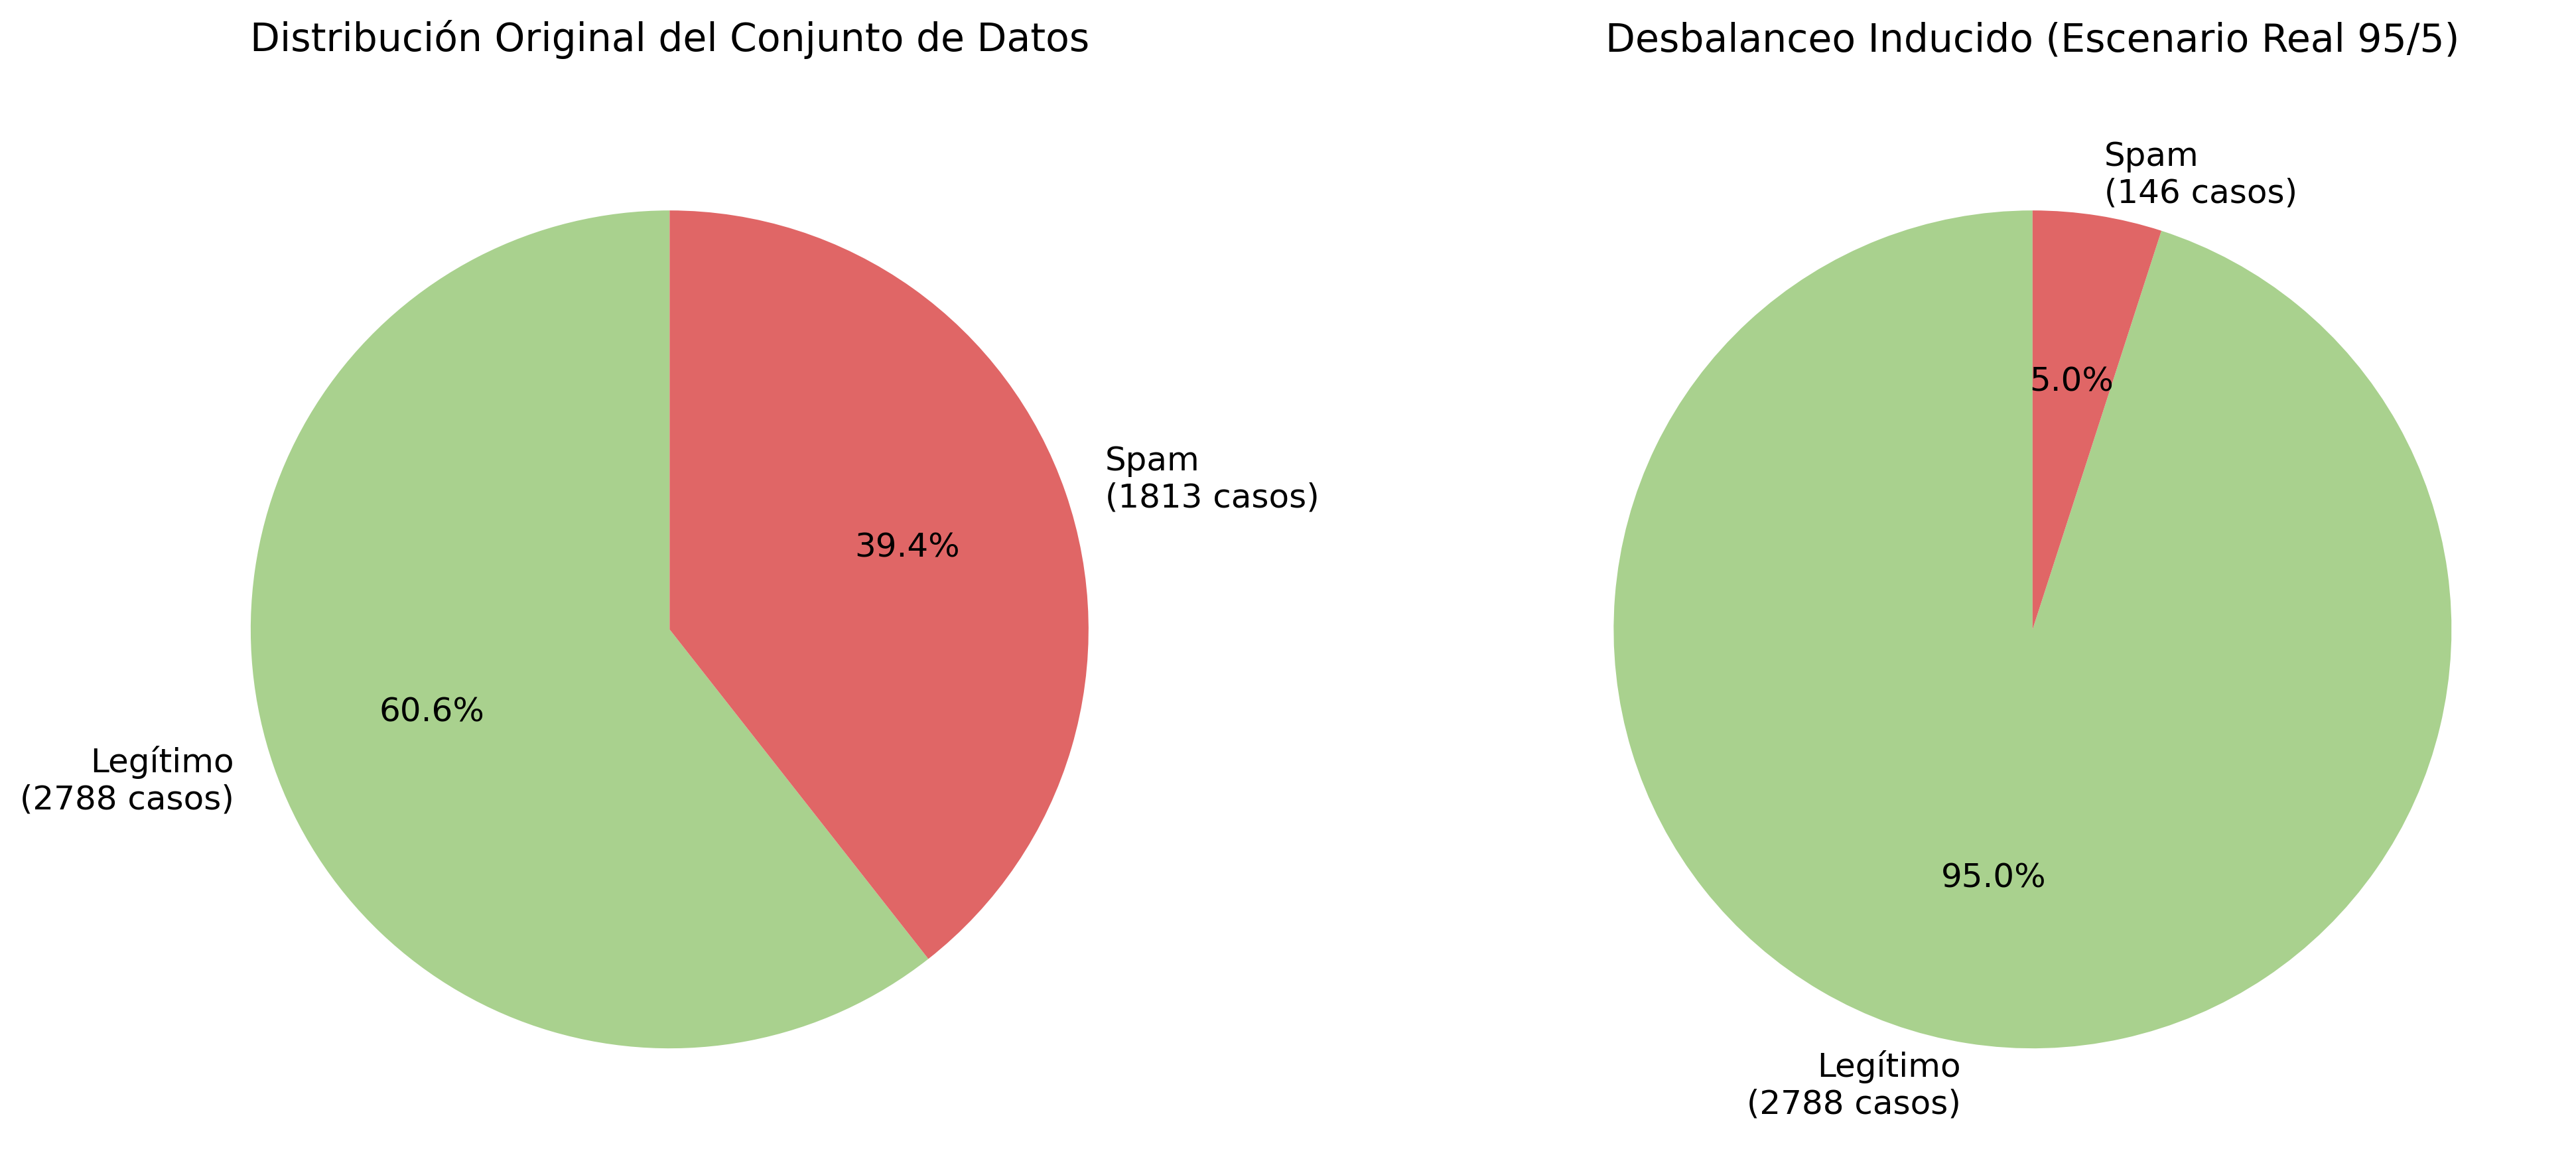
\includegraphics[width=\textwidth]{distribucion_clases.png}
    \caption{Comparación entre la distribución original de clases del conjunto de datos y la inducción de desbalanceo artificial simulando un escenario del mundo real (95\% / 5\%).}
    \label{fig:distribucion_clases}
\end{figure}

A continuación, el conjunto de datos resultante se dividió en dos subconjuntos: un 80\% de las instancias se destinó al entrenamiento de los modelos, mientras que el 20\% restante se reservó exclusivamente para las pruebas de evaluación final. 

Para evitar cualquier posible filtración de información (\textit{data leakage}) desde el conjunto de prueba hacia la fase de aprendizaje, la estandarización de las escalas numéricas se realizó de forma estricta después de la división. Se utilizó la herramienta \texttt{StandardScaler} (provista por la librería \texttt{scikit-learn}) para ajustar los valores numéricos de las variables predictoras a una media de cero y varianza de uno. Este escalador se ajustó de forma exclusiva utilizando únicamente la información de los datos de entrenamiento; Posteriormente, esas mismas reglas calculadas se utilizaron tanto para el conjunto de entrenamiento como el de prueba. Este paso de estandarización es un requisito para garantizar el correcto funcionamiento de los clasificadores basados en el cálculo de distancias geométricas.\section{Técnicas de Balanceo}
Para contrarrestar el fuerte desequilibrio de clases descrito en la sección anterior, se implementaron cuatro enfoques distintos de sobremuestreo. Estas técnicas emplean algoritmos para generar nuevas instancias sintéticas basándose en las relaciones matemáticas y geométricas de los ejemplos ya presentes en el espacio de datos. El análisis se estructuró comenzando por los algoritmos generativos clásicos, para luego avanzar hacia sus respectivas evoluciones modernas.

\section{Técnicas de Balanceo}
Para contrarrestar el fuerte desequilibrio de clases descrito en la sección anterior, se implementaron cuatro enfoques distintos de sobremuestreo. Estas técnicas emplean algoritmos para generar nuevas instancias sintéticas basándose en las relaciones matemáticas y geométricas de los ejemplos ya presentes en el espacio de datos. El análisis se estructuró comenzando por los algoritmos generativos clásicos, para luego avanzar hacia sus respectivas evoluciones modernas.

\paragraph{SMOTE (Synthetic Minority Over-sampling Technique) 
Es el algoritmo estándar a la hora de crear datos sintéticos para balancear un conjunto de datos. Funciona analizando los ejemplos de la clase minoritaria (los correos \textit{spam}) uno por uno. Para cada correo, el algoritmo busca a sus $k$ vecinos más cercanos (usualmente $k=5$). 

Una vez elegido un vecino al azar, la generación del nuevo dato sintético ($x_{nuevo}$) se realiza mediante una interpolación matemática lineal entre la instancia original ($x_i$) y su vecino ($x_{vecino}$):
\begin{equation}
x_{nuevo} = x_i + \lambda \times (x_{vecino} - x_i)
\end{equation}
donde $\lambda$ es un número aleatorio entre $0$ y $1$ que ubica al nuevo correo en un punto intermedio de la línea que los une. La cantidad de vecinos que el algoritmo conecta depende de la brecha de datos que se deba llenar. Para este estudio, donde se partió de un número extremadamente bajo de clase minoritaria (apenas el $5\%$), el algoritmo debió inyectar aleatoriedad trazando aproximadamente 7 líneas a partir de cada instancia original para alcanzar el porcentaje deseado.\cite{chawla2002smote}.}

\paragraph{ADASYN (Adaptive Synthetic) \cite{he2008adasyn}.}
La principal diferencia y ventaja de ADASYN frente a SMOTE es que presta mucha más atención a la  zona donde las clases se mezclan entre si y son dificiles de separar. 

Para lograr esto, el algoritmo primero calcula la distribución de densidad de la clase mayoritaria alrededor de cada ejemplo de la clase minoritaria. Con esa información, calcula un "ratio de dificultad" de aprendizaje para cada instancia. Luego, procede a crear una mayor cantidad de datos artificiales \textit{únicamente} alrededor de los ejemplos que resultaron ser más conflictivos de clasificar. De esta manera, el modelo concentra su esfuerzo en la frontera límite, evitando generar información innecesaria en zonas seguras que el clasificador ya domina.\cite{he2008adasyn}.}

\paragraph{G-SMOTE (Geometric SMOTE) 
Es una evolución geométrica directa del algoritmo SMOTE original. El problema del enfoque clásico de SMOTE es que crea los datos nuevos estrictamente sobre líneas rectas, lo que puede generar confusion al clasificador si esas líneas cruzan cerca de la clase contraria. 

G-SMOTE soluciona esto definiendo una zona esférica alrededor de las instancias originales de la clase minoritaria, generando las nuevas muestras en cualquier punto dentro de ese volumen hiperespacial. La clave que hace a este algoritmo tan seguro y preciso es cómo define el tamaño de su esfera: antes de crearla, calcula la distancia euclidiana exacta hacia el ejemplo de la clase mayoritaria más cercano, y restringe el radio de generación para no cruzar nunca esa distancia límite. Esto permite crear ejemplos sumamente variados con la garantía matemática de que no invadirán el territorio de los correos legítimos.\cite{douzas2019gsmote}.}

\paragraph{ADASYN + ENN 
Este método híbrido combina la creación  de datos de ADASYN con una  etapa de limpieza algorítmica llamada \textit{Edited Nearest Neighbours} (ENN). 

El proceso consta de dos fases. Primero, ADASYN inyecta nuevos datos sintéticos en las zonas más difíciles de clasificar para reforzar la presencia de la amenaza. Segundo, el algoritmo ENN revisa todo el conjunto de datos ampliado evaluando a los vecinos más cercanos (típicamente empleando $k=3$) de cada observación. Si detecta que un ejemplo (ya sea un correo real o uno sintético recién creado) tiene una mayoría de vecinos pertenecientes a la clase contraria, asume que es un dato  que confundirá al clasificador y lo elimina por completo. La sinergia de estos dos pasos permite entregarle al modelo unos datos de entrenamiento robustos pero excepcionalmente limpios.\cite{batista2004study}.}

\vspace{0.5cm}
\noindent Inicialmente se buscó igualar el conjunto a una proporción exacta de 50/50, pero se evidenció que este exceso de ejemplos sintéticos provocaba que muchos correos legítimos fueran erróneamente clasificados como \textit{spam}. Durante las pruebas de ajuste, se observó que balancear los datos hasta lograr una relación aproximada del $70\%$ de correos legítimos y un $30\%$ de \textit{spam} arrojaba los mejores resultados globales. Esta proporción logró el equilibrio perfecto: permitió que los algoritmos aprendieran a detectar las amenazas con alta eficacia, manteniendo al mismo tiempo un control sobre la tasa de falsos positivos.
\begin{figure}[htbp]
    \centering
    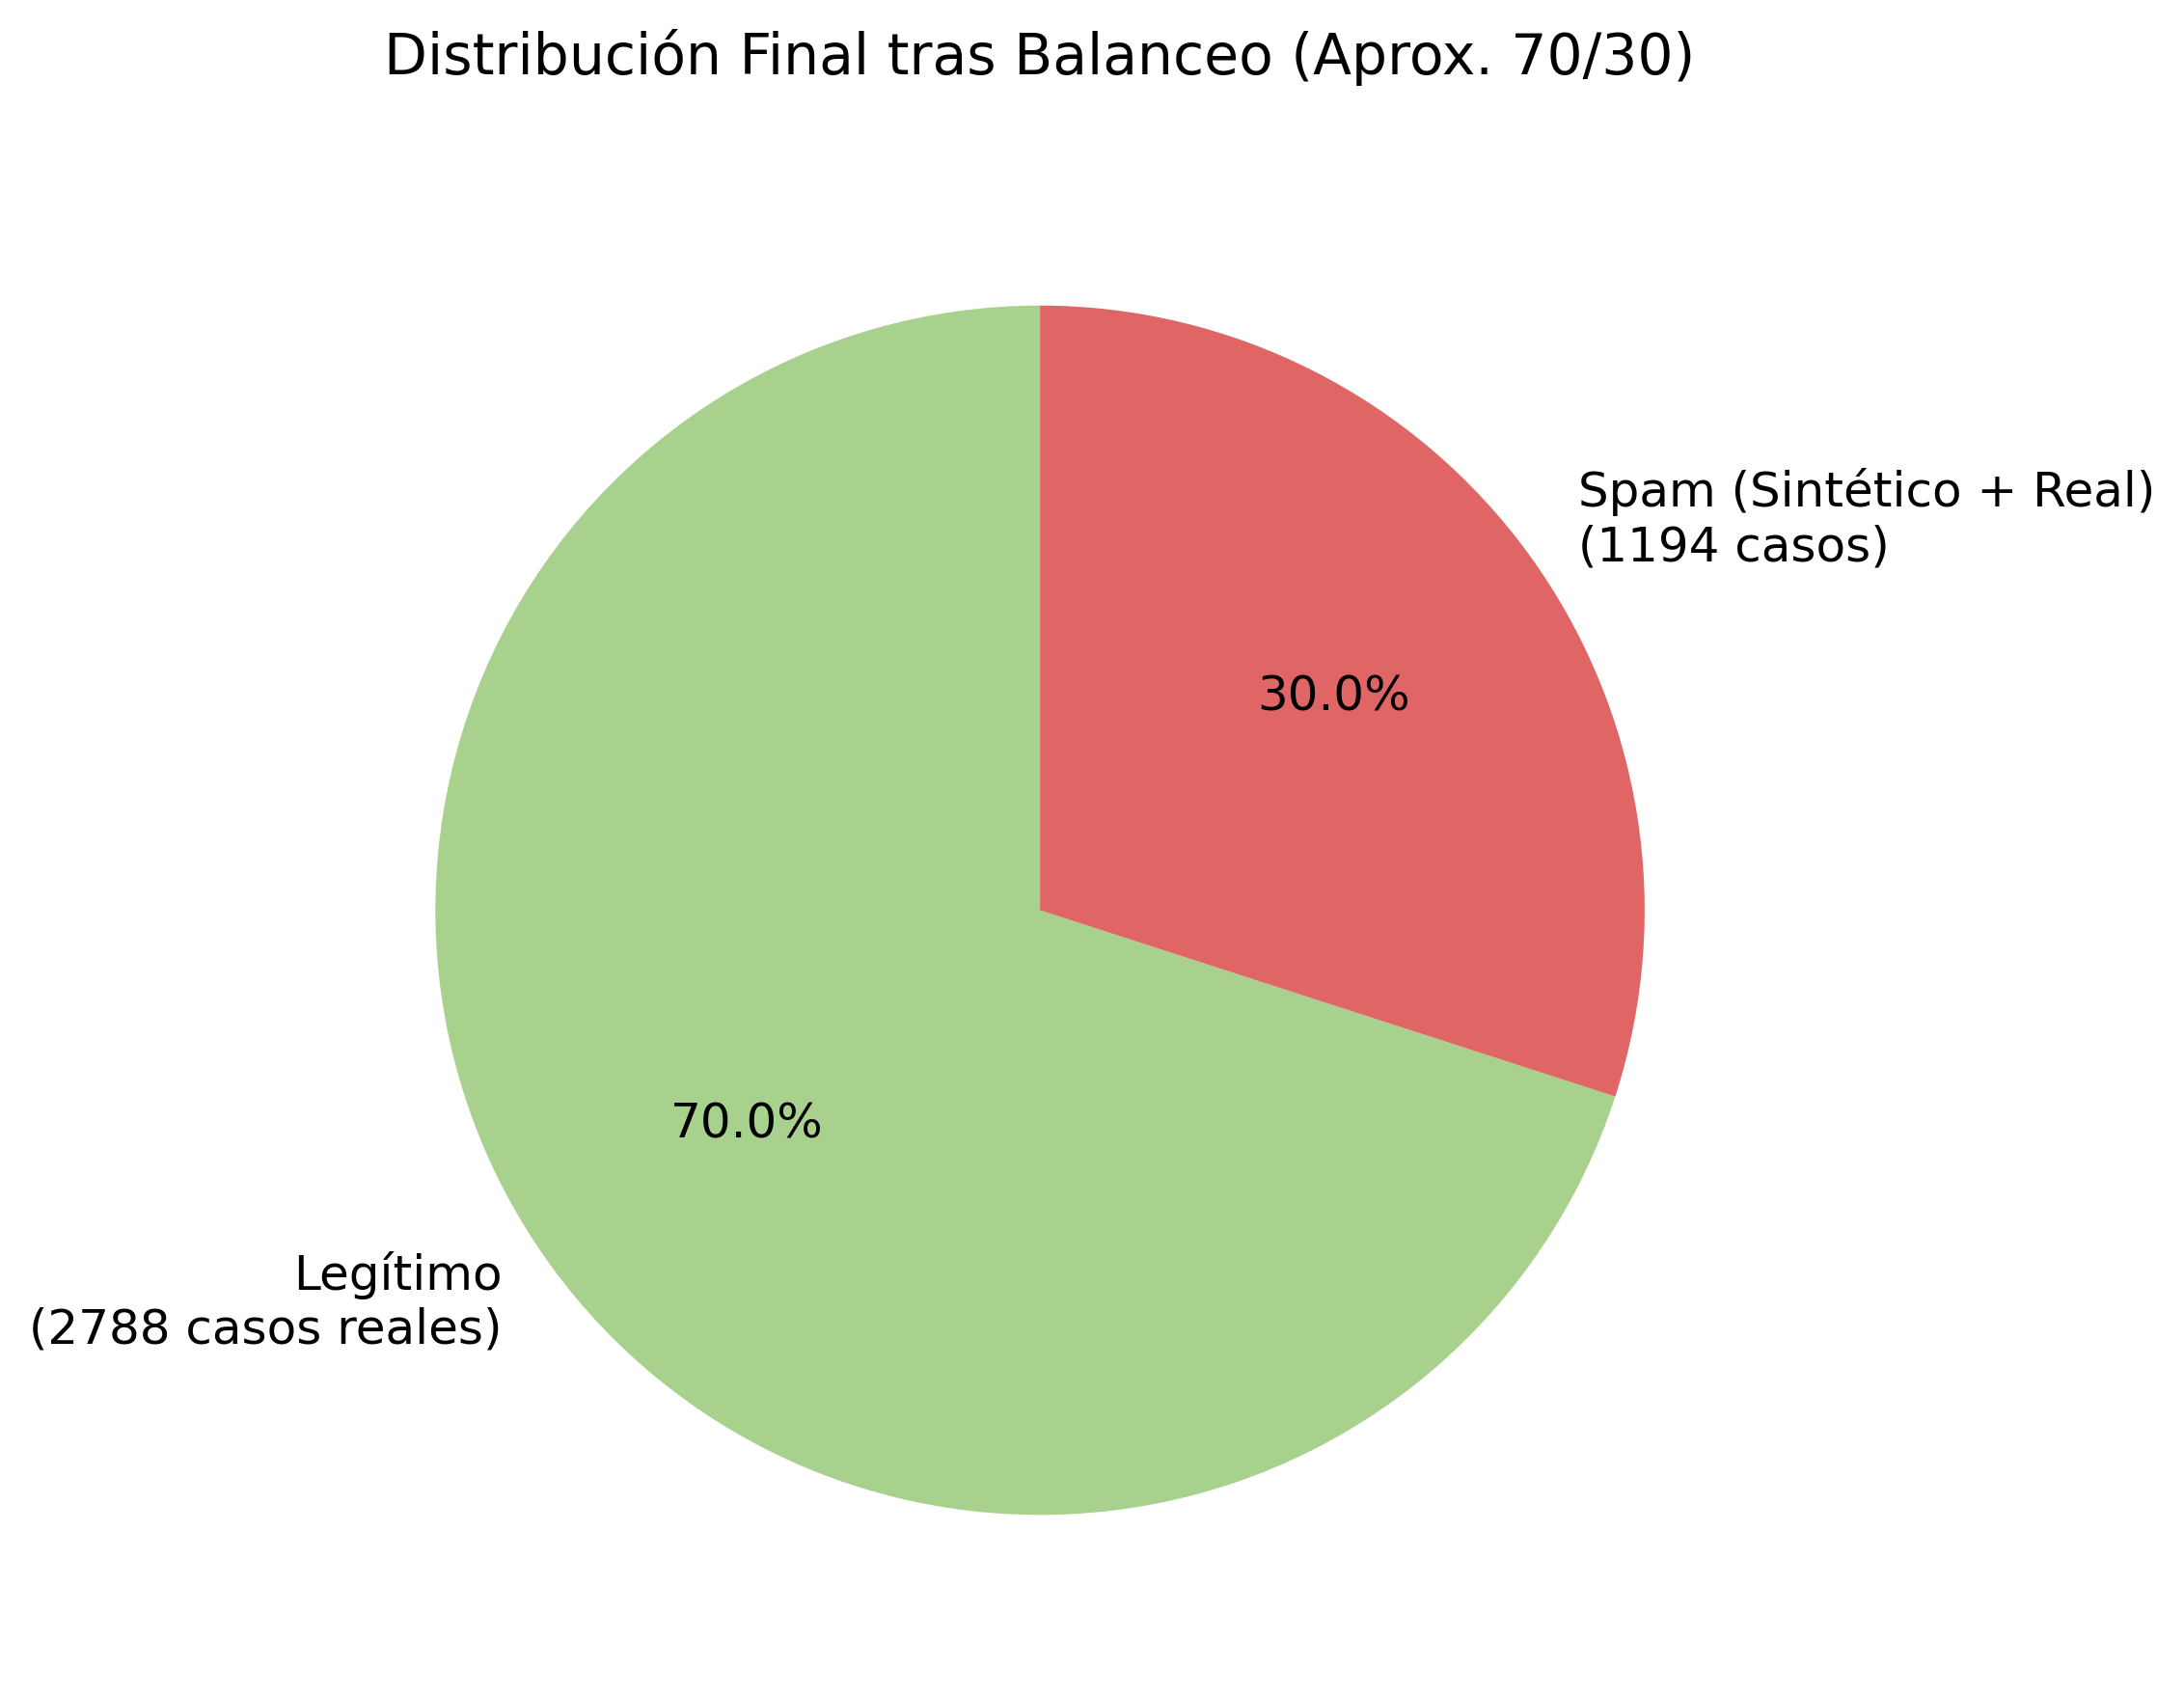
\includegraphics[width=0.7\textwidth]{distribucion_balanceada.png}
    \caption{Distribución final del conjunto de datos de entrenamiento tras aplicar las técnicas de sobremuestreo (relación aproximada 70/30).}
    \label{fig:distribucion_balanceada}
\end{figure}


\section{Modelos de Clasificación Seleccionados}

Una vez que los datos fueron debidamente preprocesados y balanceados, se procedió a entrenar y evaluar tres modelos clásicos de aprendizaje automático. Para mantener el enfoque en el análisis del balanceo de datos, se utilizaron las configuraciones predeterminadas de los algoritmos (provistas por la librería \texttt{scikit-learn}), a excepción de un ajuste particular en uno de los modelos que se detalla más adelante.

\paragraph{Árboles de Decisión.} El aprendizaje por Árboles de Decisión es un método no paramétrico que funciona creando divisiones jerárquicas mediante una secuencia de preguntas lógicas del tipo (\textit{if-else}). 

El objetivo de este algoritmo es encontrar la partición que separe la clase positiva de la negativa de la forma más limpia posible. Cada vez que el árbol hace una pregunta sobre una característica (por ejemplo, evaluar si un valor supera cierto umbral), el conjunto de datos se divide en sub-nodos. El modelo evaluará estas divisiones buscando siempre alcanzar "nodos puros"; es decir, hojas finales que contengan exclusivamente instancias de una sola clase. 

Para medir la bondad de cada partición y elegir la mejor pregunta, el algoritmo minimiza funciones matemáticas de impureza, como el índice de Gini. Este índice mide la frecuencia con la que un ejemplo sería clasificado incorrectamente si se lo etiquetara de forma aleatoria. Para un nodo $t$, se calcula como:
\begin{equation}
\text{Gini}(t) = 1 - \sum_{k=1}^{K} \left( p(k|t) \right)^2
\label{eq:gini}
\end{equation}
donde $K$ es el número total de clases (en este caso, \textit{spam} o legítimo) y $p(k|t)$ representa la proporción de ejemplos que pertenecen a una clase específica dentro de ese nodo. El valor del índice es $0$ cuando el nodo es perfectamente puro (todos los correos son de la misma clase) y aumenta a medida que los correos \textit{spam} y legítimos están más mezclados.

\paragraph{Bosques Aleatorios (Random Forest).} El algoritmo de Random Forest (Bosque Aleatorio) implementa un proceso conocido como \textit{Bagging} (\textit{Bootstrap Aggregating}). En lugar de construir un solo árbol, este método construye múltiples árboles independientes. La clave de su éxito radica en el uso de dos procesos aleatorios durante su creación:
\begin{enumerate}
    \item \textbf{Bootstrap:} Cada árbol se entrena con una muestra aleatoria distinta de los correos originales (con reemplazo).
    \item \textbf{Selección de atributos:} Al momento de hacer las preguntas \textit{if-else}, cada árbol solo puede evaluar un subconjunto aleatorio de las variables. Esto genera muchos árboles con distintas evaluaciones que servirán para evaluar en un futuro las nuevas instancias sin el riesgo de que, durante la fase de entrenamiento, el clasificador se haya sobreentrenado para el conjunto de entrenamiento original.
\end{enumerate}

Finalmente, cuando llega un correo nuevo (representado matemáticamente como un vector de características $\boldsymbol{x}$), se realiza el proceso de agregación (\textit{Aggregating}): todos los árboles del bosque lo analizan individualmente y emiten su predicción. La clase final del correo ($\widehat{y}$) se decide por \textbf{voto mayoritario}, eligiendo la clase $C_l$ que reciba la mayor cantidad de votos:
\begin{equation}
\widehat{y} = \underset{C_l}{\text{argmax}} \sum_{a=1}^{A} \mathbb{I}(\widehat{y}_a(\boldsymbol{x}) = C_l)
\label{eq:rf_voting}
\end{equation}
donde $A$ es la cantidad total de árboles en el bosque y $\mathbb{I}$ es una función indicadora que suma un voto ($1$) cada vez que un árbol $a$ vota por la clase $C_l$ (ya sea \textit{spam} o legítimo). Este trabajo en equipo permite compensar los errores individuales y logra un modelo predictivo robusto y sumamente estable.

\paragraph{Máquinas de Soporte Vectorial (SVM) \textit{Support vector machine  }.} Este algoritmo aborda la clasificación buscando el hiperplano óptimo que produzca el mayor espacio posible entre las clases. A diferencia de otros métodos, la SVM no elige cualquier separación, sino que busca un \textbf{Clasificador de Margen Maximal}; es decir, el hiperplano que mejor separe los correos \textit{spam} de los legítimos basándose exclusivamente en las instancias más críticas (los vectores de soporte).
Para lidiar con correos atípicos (\textit{outliers}) y evitar el sobreajuste, la librería \texttt{scikit-learn} implementa por defecto un \textbf{margen suave}). Siguiendo los principios de este algoritmo, se sacrifica la idea de una separación perfecta (permitiendo ciertas penalidades o errores durante el entrenamiento) para lograr una mayor robustez de clasificación general.
Matemáticamente, la decisión de clasificar un nuevo correo $\boldsymbol{x}$ se toma evaluando su posición respecto a la frontera mediante la siguiente función:
\begin{equation}
f(\boldsymbol{x}) = \text{sign}\left( \sum_{i=1}^{n} \alpha_i y_i K(\boldsymbol{x}_i, \boldsymbol{x}) + b \right)
\label{eq:svm_decision}
\end{equation}
donde $K(\boldsymbol{x}_i, \boldsymbol{x})$ es la función Kernel que calcula la similitud geométrica entre el correo nuevo y los vectores de soporte del entrenamiento, $\alpha_i$ son unos coeficientes que le otorgan peso exclusivamente a esos vectores críticos, $y_i$ son las etiquetas conocidas de las clases y $b$ determina el desplazamiento de la frontera. Si el resultado de la función $f(\boldsymbol{x})$ es positivo, el modelo asigna el correo a la clase positiva; si es negativo, a la clase negativa.

\vspace{0.5cm}
\noindent \textbf{Optimización de Hiperparámetros mediante Grid Search}

Para garantizar el máximo rendimiento de la Máquina de Soporte Vectorial, no se utilizaron valores arbitrarios para su configuración interna. Por el contrario, se implementó una búsqueda exhaustiva en cuadrícula (\textit{Grid Search}) combinada con validación cruzada. 

Este método automatizado entrena y evalúa el modelo múltiples veces, probando sistemáticamente todas las combinaciones posibles de un conjunto de hiperparámetros predefinidos. El objetivo de este riguroso proceso computacional es encontrar la configuración exacta que minimice el error de clasificación general. En la Tabla \ref{tab:svm_grid} se detallan los rangos de valores explorados para cada hiperparámetro durante la fase de optimización.

\begin{table}[htbp]
\centering
\caption{Grilla de hiperparámetros evaluados y ajustados para el modelo SVM.}
\label{tab:svm_grid}
\renewcommand{\arraystretch}{1.3}
\begin{tabular}{ll}
\hline
\textbf{Parámetro} & \textbf{Valores Evaluados} \\
\hline
\texttt{C} (Parámetro de regularización) & $0.001$, $0.01$, $0.1$, $1$, $10$, $15$, $20$, $25$ \\
\texttt{kernel} (Tipo de frontera) & \texttt{linear}, \texttt{poly}, \texttt{rbf}, \texttt{sigmoid} \\
$\gamma$ (\texttt{gamma}) (Influencia local) & \texttt{scale}, \texttt{auto}, $0.001$, $0.01$, $0.1$, $1$ \\
\texttt{degree} (Grado polinómico) & $2, 3, \dots, 10$ \\
\textbf{Umbral de Decisión (\textit{Threshold})} & \textbf{0.5 (Por defecto), 0.2 (Optimizado)} \\
\hline
\end{tabular}
\end{table}

Finalmente, luego de la búsqueda iterativa, se concluyó que los mejores parámetros matemáticos para este conjunto de datos en particular resultaron ser idénticos a los provistos por la librería por defecto. Tras comprobar esto, se optó por ajustar manualmente el umbral de decisión a $0.2$, volviéndolo mucho más riguroso con los correos no deseados. Esta decisión se fundamenta en que es preferible que el usuario tenga que buscar esporádicamente en su carpeta de \textit{spam} un correo de un aviso de pago extraviado, a que, por mantener un filtro permisivo, caiga víctima de un ataque de \textit{phishing}.



\label{ch:resultados}


% --- GRÁFICOS DE RESULTADOS ---
\begin{figure}[htbp]
    \centering
    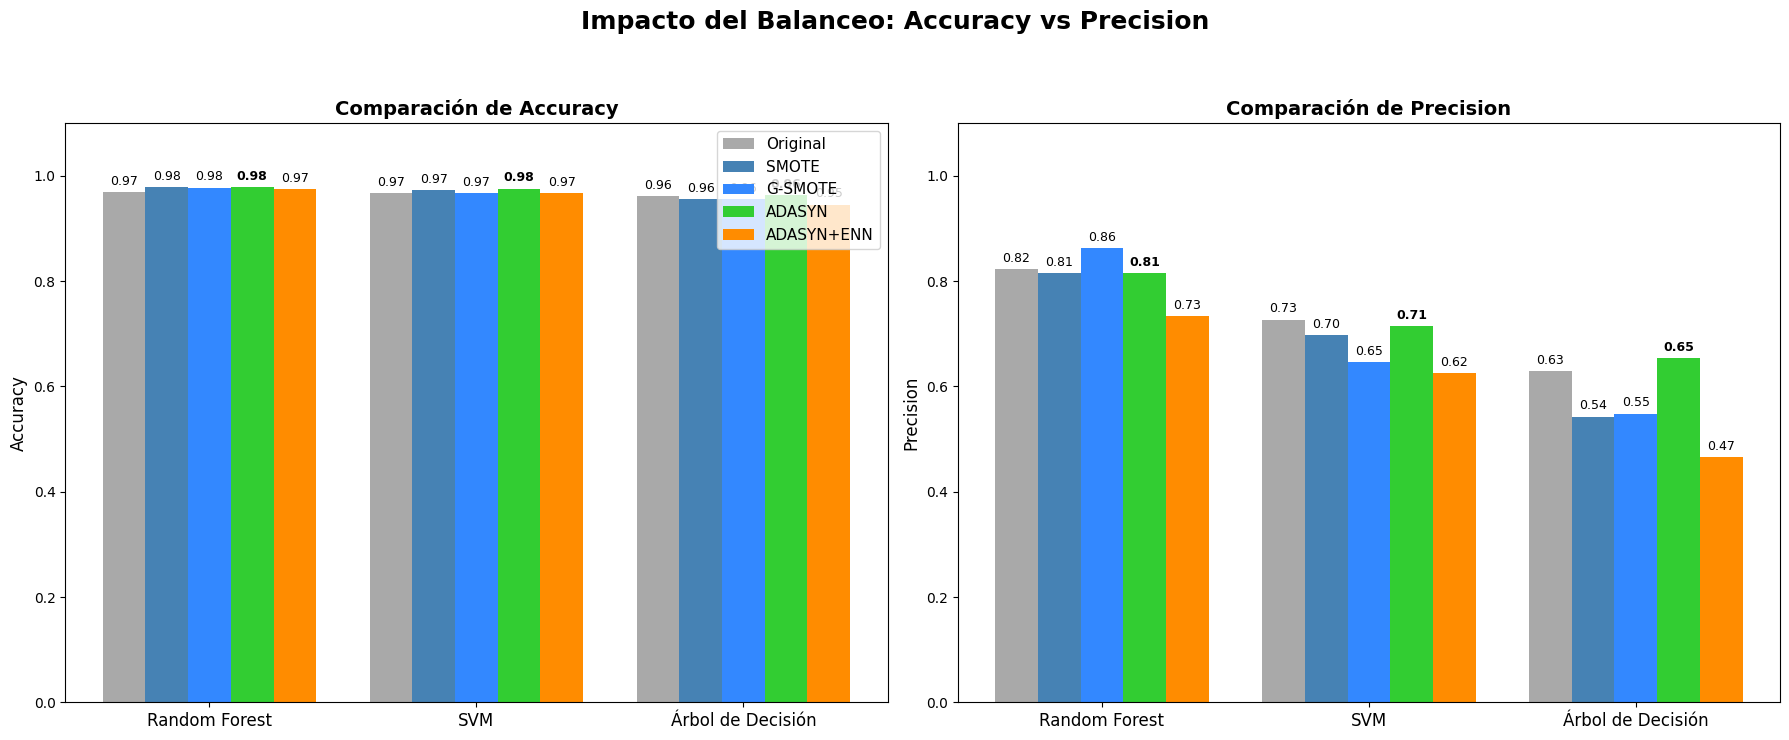
\includegraphics[width=\textwidth]{accuracy_y_precision.png}
    \caption{Impacto de las técnicas de sobremuestreo en las métricas de Accuracy y Precision para los distintos modelos evaluados.}
    \label{fig:acc_prec}
\end{figure}
\begin{figure}[htbp]
    \centering
    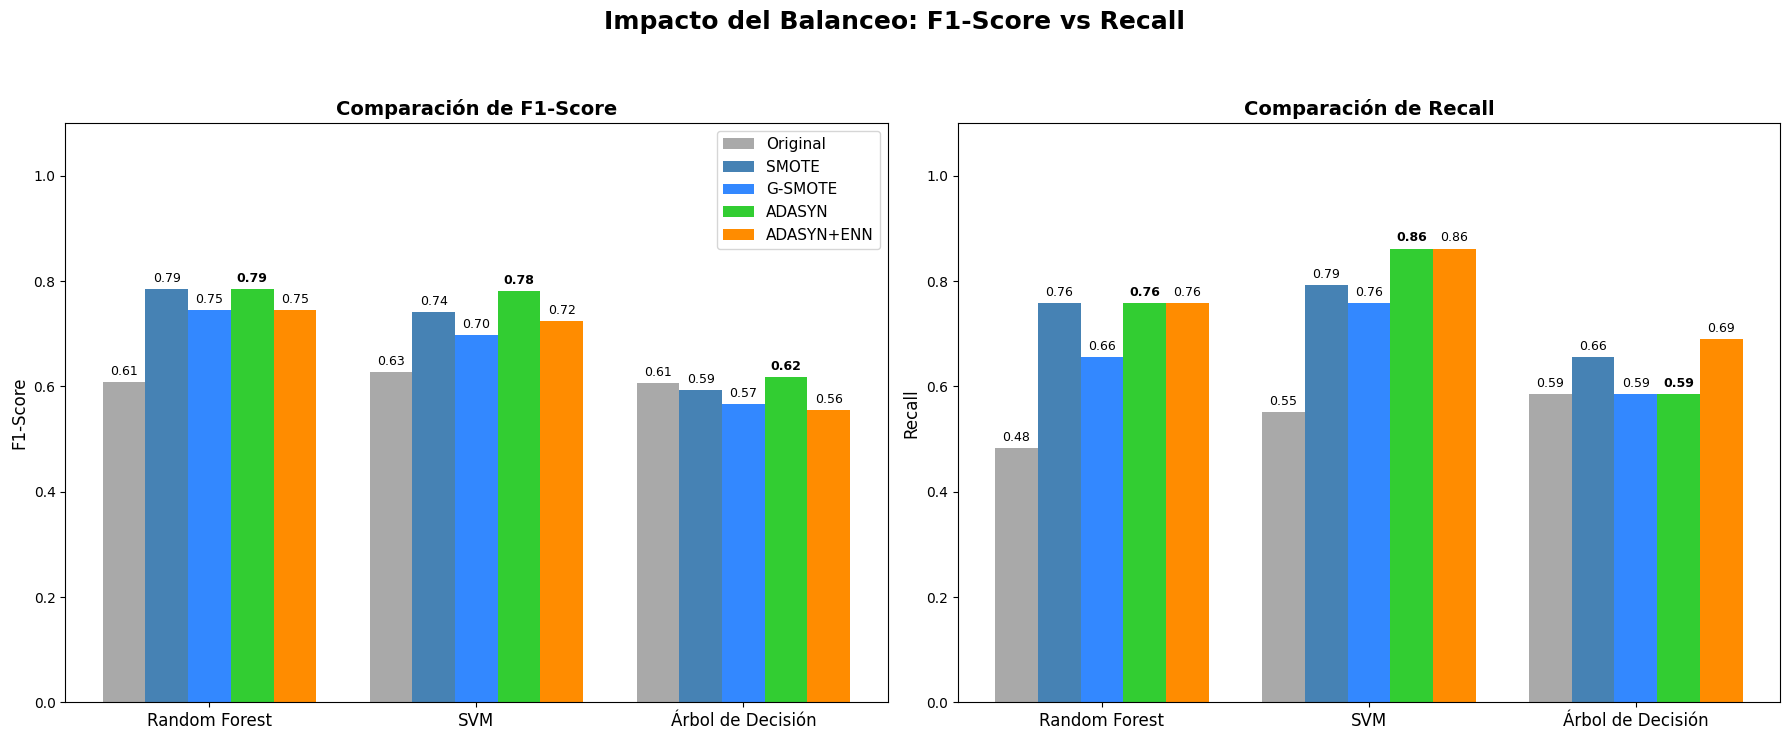
\includegraphics[width=\textwidth]{f1_y_recall.png}
    \caption{Impacto de las técnicas de sobremuestreo en las métricas de F1-Score y Recall. Se observa la superioridad de ADASYN en la métrica de Recall para el modelo SVM.}
    \label{fig:f1_recall}
\end{figure}


\chapter{Conclusiones}

\bibliographystyle{unsrt}
\bibliography{Referencias}
\addcontentsline{toc}{chapter}{Bibliografía}

\end{document}
